\documentclass[a4paper,USenglish,cleveref,autoref,thm-restate]{lipics-v2021}
% Add the option "anonymous" for a double-blind submission.

\pdfoutput=1
\hideLIPIcs

\bibliographystyle{plainurl}

\usepackage{amssymb}
\usepackage{mathtools}
\usepackage{stmaryrd}
\usepackage{tikz}
\usetikzlibrary{arrows.meta,calc,decorations.pathreplacing,positioning,fit,backgrounds}

% ---------- general ----------
\newcommand{\nat}{\mathbb{N}}
\newcommand{\defeq}{\mathrel{\vcentcolon=}}
\newcommand{\set}[1]{\{#1\}}
\newcommand{\range}[1]{[#1]}
\newcommand{\card}[1]{\lvert #1\rvert}

% ---------- terms ----------
\newcommand{\compo}{\mathbin{;}}
\newcommand{\union}{\cup}
\newcommand{\inter}{\cap}
\newcommand{\com}[1]{\overline{#1}}
\newcommand{\emp}{\emptyset}
\newcommand{\id}{\mathsf{1}}
\newcommand{\topr}{\top}
\newcommand{\Dt}{\mathsf{D}}          % strict order term
\newcommand{\St}{\mathsf{S}}          % successor term
\newcommand{\Kt}{\mathsf{K}}
\newcommand{\Nt}{\mathsf{N}}
\newcommand{\Ht}{\mathsf{H}}
\newcommand{\Psit}{\Psi}
\newcommand{\sem}[2]{\llbracket #1\rrbracket_{#2}}
\newcommand{\sh}{\mathrm{h}}
\newcommand{\cd}{\mathrm{cd}}
\newcommand{\SF}[1]{\mathrm{SF}_{#1}}
\newcommand{\Rep}[1]{\Sigma_{#1}}
\newcommand{\gsh}[1]{\mathrm{gsh}_{#1}}

% variables
\newcommand{\vr}{r}
\newcommand{\vc}{c}
\newcommand{\vb}{b}

% ---------- structures ----------
\newcommand{\A}{\mathfrak{A}}
\newcommand{\M}{\mathfrak{M}}
\newcommand{\C}{\mathfrak{C}}
\newcommand{\RSUB}{\mathsf{RSUB}}
\newcommand{\Cls}[1]{\mathcal{C}_{#1}}
\newcommand{\Gaif}{G}
\newcommand{\pw}{\mathrm{pw}}
\newcommand{\succrel}{\mathrm{succ}}
\newcommand{\tp}[1]{\mathrm{tp}_{#1}}
\newcommand{\Spec}[1]{\mathrm{Spec}_{#1}}
\newcommand{\eqq}[1]{\approx_{#1}}
\newcommand{\Obs}[1]{\mathcal{L}_{#1}}

% branches
\newcommand{\bg}{\mathtt{g}}
\newcommand{\bs}{\mathtt{s}}
\newcommand{\bl}{\mathtt{l}}
\newcommand{\Bad}{\mathtt{Bad}}
\newcommand{\pc}{\mathrm{pc}}
\newcommand{\scode}{\mathrm{sc}}

% monoids
\newcommand{\Pm}{\mathbb{P}}
\newcommand{\Qm}{\mathbb{Q}}
\newcommand{\Tm}{\mathbb{T}}
\newcommand{\Kid}{K}
\newcommand{\Types}[1]{\mathbb{W}_{#1}}

% logic
\newcommand{\FO}{\mathrm{FO}}
\newcommand{\MSO}{\mathrm{MSO}}
\newcommand{\MOD}[1]{\mathrm{MOD}_{#1}}



\crefname{claim}{Claim}{Claims}
\Crefname{claim}{Claim}{Claims}

\title{Generalized Star Height Two Is Needed on Valuations of Pathwidth Two}
\titlerunning{Generalized Star Height Two on Pathwidth Two}

\author{Yoshiki Nakamura}{Chiba University, Japan}{nakamura.yoshiki.ny@gmail.com}{https://orcid.org/0000-0003-4106-0408}{}
\authorrunning{Y. Nakamura}
\Copyright{Yoshiki Nakamura}

\ccsdesc[500]{Theory of computation~Formal languages and automata theory}
\ccsdesc[300]{Theory of computation~Finite Model Theory}
\ccsdesc[300]{Theory of computation~Logic and verification}

\keywords{Kleene algebra with complement, generalized star height, calculus of relations, pathwidth, Ehrenfeucht--Fra\"iss\'e games, finite monoids}

\category{}
\relatedversion{}
% \funding{}  % TODO

\nolinenumbers

\begin{document}

\maketitle

\begin{abstract}
We study the generalized star height of terms of Kleene algebra with complement, interpreted over $\RSUB$, the finite relational models in which variables denote forward relations on finite linear orders.
We ask how simple the underlying structures can be while height one and height two are still separated.
We measure simplicity by the pathwidth of the Gaifman graph of a valuation together with the successor relation of the order.
Pathwidth one essentially means words, and there the question is closely related to the open generalized star-height problem for regular languages.
We show that pathwidth two already suffices for a separation.
We give a fixed term $\Psi$ of star height two over three variables that is not equivalent to any term of star height at most one on the class of $\RSUB$ valuations of pathwidth at most two.
The counter-models are very simple: their Gaifman graphs are paths with a few fans attached.
On pathwidth one, $\Psi$ itself is equivalent to a term of star height one, so the bound two is tight for $\Psi$.
The proof combines Ehrenfeucht--Fra\"iss\'e games with an aperiodic and a non-aperiodic finite monoid.
These give, for every depth, two modules that no star of that depth can tell apart, while a single nested star reads a parity bit from them.
A replacement lemma and a parity argument for first-order logic with modular predicates then rule out all terms of star height one.

\end{abstract}

\section{Introduction}\label{section: introduction}

The \emph{star height} of a regular expression is the maximal nesting depth of Kleene stars in it~\cite{egganTransitionGraphsStarheight1963}.
When complement is admitted as an operator, one speaks of \emph{generalized} star height.
Languages of generalized star height $0$ are exactly the star-free languages~\cite{schutzenbergerFiniteMonoidsHaving1965}.
It is a long-standing open problem whether some regular language has generalized star height at least two~\cite{pinResultsGeneralizedStarheight1992}.
Recently, OpenAI announced a proof that every regular language has generalized star height at most three~\cite{openaiGeneralizedStarHeight2026}.

The same question can be asked for \emph{terms} of Kleene algebra with complement, that is, for expressions over variables.
Here the variables are interpreted as binary relations, and two terms are compared by their values under all valuations in a class of models.
This viewpoint goes back to Tarski's calculus of relations~\cite{tarskiCalculusRelations1941} and its extension with transitive closure~\cite{ngRelationAlgebrasTransitive1984}.
We work with $\RSUB$~\cite{nakamuraFiniteRelationalSemantics2025}.
In $\RSUB$, the universe is a finite linear order, each variable denotes a set of forward pairs, and complement is taken relative to the set of all forward pairs.
$\RSUB$ captures the equational theory of Kleene algebra with complement with respect to languages~\cite{nakamuraFiniteRelationalSemantics2025}.

In this paper we ask \emph{how simple the structures can be} if generalized star height one and two are still to be separated.
We measure structural simplicity by pathwidth.
To a valuation we associate its Gaifman graph, in which we also include the successor relation of the underlying linear order.
The successor relation is star-free definable from the order, so this is a natural choice.
Let $\Cls{k}$ be the class of $\RSUB$ valuations whose graph has pathwidth at most $k$.
\begin{itemize}
  \item On $\Cls{1}$, every input pair is a loop or a successor pair, since any other pair closes a cycle with the successor path.
        So a valuation in $\Cls{1}$ is essentially a word whose letters record which variables hold on each successor pair.
        The separation of heights one and two on $\Cls{1}$ is therefore closely related to the classical open problem (\Cref{remark: pathwidth one words}).
  \item Our main result shows that one more unit of pathwidth suffices for a separation.
\end{itemize}

\begin{theorem}[Main theorem]\label{theorem: main}
  There is a term $\Psit$ over three variables with star height two such that no term of star height at most one is equivalent to $\Psit$ on $\Cls{2}$.
  In other words, the generalized star height of $\Psit$ relative to $\Cls{2}$ is exactly two.
\end{theorem}

The term $\Psit$ is defined in \eqref{equation: Psi}.
It is fixed in advance, and only the counter-models depend on the competing term.
The counter-models have a very simple shape (\Cref{figure: module,figure: cells}).
Their graphs consist of a single path, together with a few vertices that are joined to some later vertices of their own segment of the path.
So each segment forms a fan, and the whole graph is a chain of fans.
Such graphs are outerplanar and have pathwidth exactly two.
The bound two is tight for this witness.
On $\Cls{1}$, the term $\Psit$ is equivalent to a term of star height one (\Cref{proposition: pathwidth one}).

\subparagraph*{Idea of the proof.}
The term $\Psit$ has the form $\Ht^*$.
Here $\Ht$ is a star-free combination of a relation $\Kt$ and its complement $\Nt$ inside a fixed relation $\vb$, and $\Kt$ contains the star $(\vr \compo \vr)^*$.
The counter-models are sequences of \emph{cells}.
Each cell contains a \emph{module}, that is, an interval $[u, v]$ with $(u, v) \in \vb$.
The inner star decides whether $(u, v)$ belongs to $\Kt$ by reading the parity of the length of an $\vr$-chain.
The outer star composes the cells, and the cells act as the identity or as a swap on two ports.
So $\Psit$ computes the parity of the number of cells whose module lies in~$\Kt$.

For a competing term $E$ of star height one, let $q$ bound the composition depth of the bodies of its stars.
We construct two modules $\M^{+}_q$ and $\M^{-}_q$ on the same set of vertices (\Cref{proposition: local pair}).
They differ in a single input pair, and $(u, v) \in \Kt$ holds in $\M^{+}_q$ but not in $\M^{-}_q$.
Still, no star of depth at most $q$ can tell them apart.
To construct them, we encode prefixes of a module by first-order types and suffixes by a finite automaton.
The first-order types form an aperiodic monoid, while the automaton may count modulo a number.
An idempotent in the minimal ideal of the product monoid lets us rewind both components at the same time (\Cref{section: local}).
A replacement lemma then shows that every star in $E$ is blind to the modules strictly between its endpoints (\Cref{section: replacement}).
Hence $E$ translates into first-order logic with modular predicates over the sequence of cell bits.
That logic cannot express parity, so $E$ differs from $\Psit$ (\Cref{section: lower bound}).

\subparagraph*{Related work.}
For regular languages, the generalized star-height problem is discussed in~\cite{pinResultsGeneralizedStarheight1992}.
Inside generalized star height zero, the dot-depth hierarchy is infinite~\cite{brzozowskiDotdepthHierarchyStarfree1978,thomasConcatenationGameDotdepth1987}.
% TODO: cite the companion result on the star-height hierarchy of terms w.r.t. languages / RSUB, if appropriate.
Terms of Kleene algebra with complement can be read as formulas of transitive closure logic with three variables.
For transitive closure logic on finite structures, Gr\"adel and McColm proved hierarchy theorems for the nesting of transitive closure and negation~\cite{gradelHierarchiesTransitiveClosure1996}.
On ordered finite structures, every formula of transitive closure logic is equivalent to one with a single transitive closure, at the price of higher arity~\cite{immermanLanguagesThatCapture1987}.
So the bounded arity of terms is essential here.
Expressive-power results for relational calculi via Ehrenfeucht--Fra\"iss\'e games include~\cite{nakamuraExpressivePowerSuccinctness2022}.
Our use of an idempotent from the minimal ideal of a finite monoid is standard in the algebraic theory of regular languages~\cite{pinVarietiesFormalLanguages1986}.

\subparagraph*{Organization.}
\Cref{section: preliminaries} fixes notation.
\Cref{section: overview} defines $\Psit$ and outlines the proof of \Cref{theorem: main}.
\Cref{section: modules,section: local,section: cells,section: replacement,section: lower bound} contain the proof.
\Cref{section: pathwidth one} treats pathwidth one, and \Cref{section: conclusion} concludes.

\section{Preliminaries}\label{section: preliminaries}

For $n \in \nat$ we write $\range{n} \defeq \set{1, \dots, n}$.
For a finite linear order $(V, <)$ and $x \le y$, let $\range{x, y} \defeq \set{z \mid x \le z \le y}$.
We write $\succrel$ for the successor relation of $(V, <)$.

\subparagraph*{Terms and $\RSUB$.}
We fix the variables $\vr, \vc, \vb$.
(The lower bound also holds for terms over any finite set of variables, see \Cref{remark: more variables}.)
\emph{Terms} are generated by
\[
  E, F \;::=\; x \mid \emp \mid \id \mid E \union F \mid \com{E} \mid E \compo F \mid E^{*}
  \qquad (x \in \set{\vr, \vc, \vb}).
\]
A \emph{valuation} $\A$ consists of a finite nonempty linear order $(V, <)$ and relations $\vr^{\A}, \vc^{\A}, \vb^{\A}$ contained in the set $\topr_V \defeq \set{(x, y) \in V^2 \mid x \le y}$ of \emph{forward pairs}.
It is an \emph{$\RSUB$ valuation} if each $x^{\A}$ contains either all pairs $(z, z)$ or none of them~\cite{nakamuraFiniteRelationalSemantics2025}.
The value $\sem{E}{\A} \subseteq \topr_V$ is defined as usual.
The constant $\id$ denotes the identity, $\union$ union, $\compo$ relational composition, and ${}^{*}$ reflexive transitive closure.
Complement is taken relative to $\topr_V$: $\sem{\com{E}}{\A} \defeq \topr_V \setminus \sem{E}{\A}$.
Every value consists of forward pairs.
We write $E(x, y)$ for $(x, y) \in \sem{E}{\A}$ when $\A$ is clear.
We use the abbreviations
\[
  E \inter F \defeq \com{\com{E} \union \com{F}},\quad
  E \setminus F \defeq E \inter \com{F},\quad
  \topr \defeq \com{\emp},\quad
  \Dt \defeq \com{\id},\quad
  \St \defeq \Dt \setminus (\Dt \compo \Dt),
\]
and $E^{2} \defeq E \compo E$.
Then $\Dt$ denotes the strict order $<$ and $\St$ denotes $\succrel$.
All of these abbreviations are star-free.

For $x \le y$, let $\A\range{x, y}$ be the valuation induced on $\range{x, y}$.
Every intermediate point of a composition, and every point on a closure path, between $x$ and $y$ lies in $\range{x, y}$.
An induction on terms gives:

\begin{lemma}[Interval locality]\label{lemma: locality}
  For every term $E$, valuation $\A$ and $x \le y$: $(x, y) \in \sem{E}{\A}$ iff $(x, y) \in \sem{E}{\A\range{x, y}}$.
\end{lemma}

\subparagraph*{Star height.}
The \emph{star height} $\sh(E)$ is the nesting depth of ${}^{*}$ in $E$.
Complement and the other operators do not count.
So $\sh(x) = \sh(\emp) = \sh(\id) = 0$, $\sh(\com{E}) = \sh(E)$, $\sh(E \union F) = \sh(E \compo F) = \max(\sh(E), \sh(F))$, and $\sh(E^*) = \sh(E) + 1$.
For a class $\mathcal{C}$ of valuations, $E$ and $F$ are \emph{equivalent on $\mathcal{C}$} if $\sem{E}{\A} = \sem{F}{\A}$ for all $\A \in \mathcal{C}$.
The \emph{generalized star height of $E$ relative to $\mathcal{C}$}, written $\gsh{\mathcal{C}}(E)$, is the least $\sh(F)$ over all $F$ equivalent to $E$ on $\mathcal{C}$.

\subparagraph*{Pathwidth.}
A \emph{path decomposition} of a graph $G$ is a sequence of \emph{bags} $X_1, \dots, X_\ell \subseteq V(G)$ with the following properties.
Every edge is contained in some bag, and for every vertex, the bags containing it form a nonempty interval.
Its width is $\max_i \card{X_i} - 1$, and the \emph{pathwidth} $\pw(G)$ of $G$ is the least width of a path decomposition of $G$~\cite{robertsonGraphMinorsExcluding1983}.
Forests have treewidth at most one, and every graph with a cycle has treewidth, and hence pathwidth, at least two.

The \emph{graph} $\Gaif(\A)$ of a valuation $\A$ has vertex set $V$.
Two distinct vertices $x, y$ are adjacent iff $(x, y)$ or $(y, x)$ belongs to $\succrel \union \vr^{\A} \union \vc^{\A} \union \vb^{\A}$.
So $\Gaif(\A)$ is the Gaifman graph of $(V, \succrel, \vr^{\A}, \vc^{\A}, \vb^{\A})$ with loops removed.
Only input relations and the successor contribute edges, and derived relations such as $\sem{\vr \compo \vr}{\A}$ do not.
We write $\pw(\A) \defeq \pw(\Gaif(\A))$ and
\[
  \Cls{k} \defeq \set{\A \mid \A \text{ is an $\RSUB$ valuation with } \pw(\A) \le k}.
\]

\subparagraph*{Star-free terms and first-order types.}
A term is \emph{star-free} if it contains no ${}^{*}$.
The \emph{composition depth} $\cd(E)$ of a star-free term is the nesting depth of $\compo$.
Thus $\cd$ is $0$ on atoms, is preserved by $\union$ and complement, and $\cd(E \compo F) = \max(\cd(E), \cd(F)) + 1$.
Let $\SF{q}$ be the set of star-free terms $E$ with $\cd(E) \le q$.
Since $\Dt$ has depth $0$, $E \in \SF{q}$ implies $E \inter \Dt \in \SF{q}$.

We regard a valuation as a first-order structure over the signature $\set{<, \vr, \vc, \vb}$.
For a structure $\mathfrak{B}$ and elements $\bar{a}$, $\tp{q}(\mathfrak{B}, \bar{a})$ denotes the first-order type of quantifier rank $q$ of $\bar a$ in $\mathfrak{B}$.
We use the Ehrenfeucht--Fra\"iss\'e characterization of these types~\cite{ehrenfeuchtApplicationGamesCompleteness1961,fraisseClassificationsSystemsRelations1954,ebbinghausFiniteModelTheory1995}.
The standard translation sends $E \compo F$ to $\exists z\,(x \le z \le y \wedge \varphi_E(x, z) \wedge \varphi_F(z, y))$.
It turns each $E \in \SF{q}$ into a first-order formula $\varphi_E(x, y)$ of quantifier rank at most $q$ with $\sem{E}{\A} = \set{(x, y) \in \topr_V \mid \A \models \varphi_E(x, y)}$.
With \Cref{lemma: locality} this gives:

\begin{lemma}\label{lemma: SF types}
  For $E \in \SF{q}$ and $x \le y$, whether $(x, y) \in \sem{E}{\A}$ holds depends only on the type $\tp{q}(\A\range{x, y}, x, y)$.
  Moreover, $\SF{q}$ contains only finitely many terms up to equivalence on all valuations.
\end{lemma}

We fix a finite set $\Rep{q} \subseteq \SF{q}$ of representatives of $\SF{q}$ up to equivalence.

\subparagraph*{Words and their types.}
Let $\Gamma$ be a finite alphabet.
A nonempty word $\alpha = \alpha_1 \cdots \alpha_k \in \Gamma^{+}$ is the structure with universe $\range{k}$, the order $<$, the successor, a unary predicate for each letter, and the constants $1$ and $k$.
Let $\tau_q(\alpha)$ be its first-order type of quantifier rank $q$.
For the empty word we add a fresh value $\tau_q(\varepsilon)$.
The following facts are standard.
We include proofs, since we need the exact thresholds.

\begin{lemma}\label{lemma: word types}
  Let $q \in \nat$.
  \begin{enumerate}
    \item\label{item: composition} If $\tau_q(\alpha) = \tau_q(\alpha')$ and $\tau_q(\beta) = \tau_q(\beta')$, then $\tau_q(\alpha\beta) = \tau_q(\alpha'\beta')$.
          Hence the values of $\tau_q$ form a finite monoid $\Types{q}(\Gamma)$, and $\tau_q \colon \Gamma^{*} \to \Types{q}(\Gamma)$ is a surjective monoid morphism.
    \item\label{item: powers} For every $\omega \in \Gamma^{+}$ and all $k, k' > 2^{q+1}$, we have $\tau_q(\omega^{k}) = \tau_q(\omega^{k'})$.
          In particular, $\Types{q}(\Gamma)$ is aperiodic.
  \end{enumerate}
\end{lemma}
\begin{proof}
  (\ref{item: composition})
  Duplicator plays the two games on $\alpha, \alpha'$ and on $\beta, \beta'$ in parallel.
  She answers each move in the part where it was made.
  The constants are matched, so the last position of $\alpha$ corresponds to the last position of $\alpha'$, and similarly for the first positions of $\beta, \beta'$.
  The only successor pair across the two parts joins the last position of $\alpha$ and the first position of $\beta$.
  So the union of the two partial isomorphisms is a partial isomorphism.
  The empty word is the identity.

  (\ref{item: powers})
  Write the positions of $\omega^{k}$ as pairs $(j, p)$, where $j \in \range{0, k-1}$ is the index of the copy and $p \in \range{\card{\omega}}$ is the position inside it.
  Duplicator always answers with the same $p$.
  She plays on the copy indices the usual strategy for linear orders~\cite{ebbinghausFiniteModelTheory1995}.
  This strategy keeps the following invariant for all pebbled elements, including the two constants.
  When $r$ rounds remain, any two copy indices have the same difference on both sides, or both differences are at least $2^{r+1}$ in absolute value, with the same sign.
  The invariant holds initially because $k-1, k'-1 \ge 2^{q+1}$.
  At the end, copy indices have equal differences or differ by at least $2$.
  Hence order, letters and the constants are preserved.
  The successor $(j, p) \to (j', p')$ requires $j' - j \in \set{0, 1}$, so it is preserved too.
  Taking $\omega$ to be a representative of an element $m \in \Types{q}(\Gamma)$ gives $m^{k} = m^{k+1}$ for $k > 2^{q+1}$.
\end{proof}

\subparagraph*{Finite monoids.}
Every finite monoid $\Tm$ has a least nonempty two-sided ideal $\Kid(\Tm)$, its \emph{minimal ideal}, and $\Kid(\Tm)$ contains an idempotent.
A monoid is \emph{aperiodic} if all its subgroups are trivial.

\begin{lemma}\label{lemma: minimal ideal}
  Let $\Tm$ be a finite monoid and $e \in \Kid(\Tm)$ an idempotent.
  \begin{enumerate}
    \item\label{item: group} $e \Tm e$ is a group with identity $e$.
    \item\label{item: collapse} If $\pi \colon \Tm \to \Pm$ is a surjective morphism onto an aperiodic monoid, then $\pi(e)\, n\, \pi(e) = \pi(e)$ for all $n \in \Pm$.
  \end{enumerate}
\end{lemma}
\begin{proof}
  (\ref{item: group})
  Let $x \in e\Tm e$.
  Since $\Tm x \Tm$ is an ideal contained in $\Kid(\Tm)$, it equals $\Kid(\Tm)$, so $e = a x b$ for some $a, b$.
  Then $e = (eae)\, x\, (ebe)$.
  In the finite monoid $e\Tm e$, a one-sided inverse is a two-sided inverse.
  So $(eae)x$ and $x(ebe)$ are invertible, and hence $x$ is invertible.

  (\ref{item: collapse})
  Since $\pi$ is surjective, $\pi(\Kid(\Tm))$ is an ideal of $\Pm$.
  Every ideal $J$ of $\Pm$ satisfies $\pi^{-1}(J) \supseteq \Kid(\Tm)$.
  So $\pi(\Kid(\Tm)) = \Kid(\Pm)$, and $\pi(e)$ is an idempotent in $\Kid(\Pm)$.
  By (\ref{item: group}), $\pi(e)\Pm\pi(e)$ is a subgroup of $\Pm$, so it is trivial.
\end{proof}

\section{The witness term and an overview of the proof}\label{section: overview}

We define
\begin{equation}\label{equation: Psi}
  \begin{aligned}
    \Kt    &\defeq \vb \inter \bigl(((\vr \compo \vr)^{*} \inter \vc) \compo \Dt\bigr), &
    \Nt    &\defeq \vb \setminus \Kt,\\
    \Ht    &\defeq (\St^{2} \compo \Kt \compo \St^{2}) \union (\St \compo \Kt \compo \St)
              \union (\St^{2} \compo \Nt \compo \St) \union (\St \compo \Nt \compo \St^{2}), &
    \Psit  &\defeq \Ht^{*}.
  \end{aligned}
\end{equation}
The star $(\vr \compo \vr)^{*}$ lies inside $\Kt$, and $\Kt$ lies inside the star $\Ht^{*}$.
All abbreviations are star-free, so $\sh(\Psit) = 2$.
Hence \Cref{theorem: main} follows from the next theorem.

\begin{theorem}\label{theorem: lower bound}
  No term $E$ with $\sh(E) \le 1$ is equivalent to $\Psit$ on $\Cls{2}$.
  This holds even if only $\RSUB$ valuations are considered in which $\vr, \vc, \vb$ are irreflexive.
\end{theorem}

The roles of the parts of $\Psit$ are as follows.
\begin{itemize}
  \item $\Kt$ reads one bit from an interval $\range{u, v}$ with $(u, v) \in \vb$, called a \emph{module}.
        The bit says whether some $\vc$-successor $y$ of $u$ can be reached from $u$ by an $\vr$-path of even length (\Cref{section: modules}).
  \item $\Ht$ shifts this bit to two ports before $u$ and two ports after $v$.
        A module in $\Kt$ swaps the ports and a module in $\Nt$ keeps them, so $\Ht^{*}$ computes a parity (\Cref{section: cells}).
\end{itemize}
Let $E$ be a term with $\sh(E) \le 1$.
Let $q$ be an upper bound of $\cd(F)$ for all subterms $F^{*}$ of $E$.
The proof of \Cref{theorem: lower bound} has three steps.
\begin{enumerate}
  \item\label{step: local pair}
        We construct two modules $\M^{+}_{q}, \M^{-}_{q}$ on the same vertices (\Cref{proposition: local pair}).
        They differ in a single $\vc$-pair, $\M^{+}_q$ is in $\Kt$ and $\M^{-}_q$ is not.
        However, no observation of the form $((A \inter \Dt) \compo F^{*} \compo (C \inter \Dt))(u, v)$ with $A, F, C \in \SF{q}$ distinguishes them.
        Note that $\Kt(u, v)$ is not of this form, since it intersects $(\vr \compo \vr)^{*}$ with $\vc$ at the pair $(u, y)$.
  \item\label{step: replacement}
        We put modules into a sequence of cells.
        A replacement lemma shows the following (\Cref{lemma: replacement}).
        For every star $F^{*}$ of $E$, replacing a module that lies strictly between the endpoints by $\M^{-}_{q}$ does not change the value of $F^{*}$.
  \item\label{step: logic}
        Hence the value of $E$ can be computed from the bit sequence of the cells by a first-order formula with modular predicates.
        That logic cannot express the parity computed by $\Psit$ (\Cref{section: lower bound}).
\end{enumerate}
Step~\ref{step: local pair} is the technical core.
The two modules must agree on all observations of depth $q$ at once.
An observation may read the prefix of a module up to some point and, at the same time, the suffix after that point.
Prefixes are described by first-order types, which form an aperiodic monoid.
Suffixes are described by a finite automaton, whose transition monoid may contain groups.
For example, $(\vr \compo \vr)^{*}$ counts modulo two.
We use an idempotent from the minimal ideal of the product monoid.
It acts as a reset on the first component and as a local identity on the second.

\section{Branches and modules}\label{section: modules}

Fix an even number $m \ge 4$.
A \emph{branch} is a chain $y_1 < \dots < y_\ell$ of length $\ell \in \set{m, m+1}$ with one \emph{selected} vertex $y_\sigma$.
We use three types of branches:
\begin{center}
  \begin{tabular}{cccc}
    type & length $\ell$ & selected index $\sigma$ & parity of $\sigma$ \\ \hline
    $\bg$ (good)    & $m$   & $m$   & even \\
    $\bs$ (shifted) & $m$   & $m-1$ & odd \\
    $\bl$ (long)    & $m+1$ & $m+1$ & odd
  \end{tabular}
\end{center}
The good type $\bg$ differs from $\bs$ only in the selected vertex, and from $\bl$ only in the length.
Let $\Bad \defeq \set{\bs, \bl}$.

\begin{definition}[Modules]\label{definition: module}
  For a nonempty word $w = t_1 \cdots t_k$ over $\set{\bg, \bs, \bl}$, the \emph{module} $\M(w)$ is the following valuation.
  Its vertices are $u$, then a branch of type $t_1$, \dots, then a branch of type $t_k$, and finally $v$, ordered from left to right.
  We set
  \begin{align*}
    \vr &\defeq \set{(u, y) \mid y \text{ is the first vertex of a branch}}\\
        &\phantom{{}\defeq{}} \union \set{(y, y') \mid y, y' \text{ are consecutive vertices of the same branch}},\\
    \vc &\defeq \set{(u, y) \mid y \text{ is the selected vertex of a branch}},
    \qquad
    \vb \defeq \set{(u, v)}.
  \end{align*}
\end{definition}

\begin{figure}[t]
  \centering
  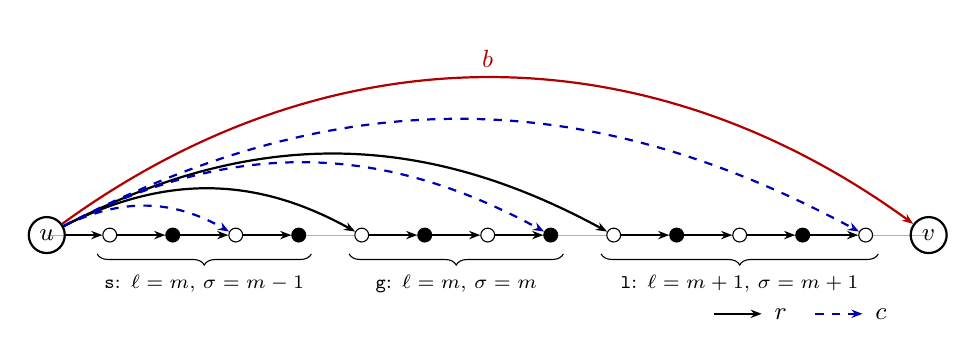
\begin{tikzpicture}[x=0.8cm,y=0.8cm,
    vtx/.style={circle,draw,inner sep=0pt,minimum size=5pt},
    even/.style={vtx,fill=black},
    odd/.style={vtx,fill=white},
    endpt/.style={circle,draw,thick,inner sep=1pt,minimum size=13pt,font=\small},
    rarr/.style={-{Stealth[length=4pt]},thick},
    carr/.style={-{Stealth[length=4pt]},dashed,thick,blue!70!black},
    barr/.style={-{Stealth[length=4pt]},thick,red!70!black},
    succ/.style={gray!60,thin}]
  % successor path
  \draw[succ] (0,0) -- (14,0);
  % endpoints
  \node[endpt] (u) at (0,0) {$u$};
  \node[endpt] (v) at (14,0) {$v$};
  % branch vertices: positions 1..13, index inside branch
  \foreach \p/\i in {1/1,2/2,3/3,4/4, 5/1,6/2,7/3,8/4, 9/1,10/2,11/3,12/4,13/5}{
    \pgfmathparse{int(mod(\i,2))}
    \ifnum\pgfmathresult=0
      \node[even] (z\p) at (\p,0) {};
    \else
      \node[odd] (z\p) at (\p,0) {};
    \fi
  }
  % r inside branches
  \foreach \a/\b in {1/2,2/3,3/4, 5/6,6/7,7/8, 9/10,10/11,11/12,12/13}{
    \draw[rarr] (z\a) -- (z\b);
  }
  % r from u to first vertices
  \draw[rarr] (u) -- (z1);
  \draw[rarr] (u) to[bend left=28] (z5);
  \draw[rarr] (u) to[bend left=28] (z9);
  % c from u to selected vertices
  \draw[carr] (u) to[bend left=28] (z3);
  \draw[carr] (u) to[bend left=28] (z8);
  \draw[carr] (u) to[bend left=28] (z13);
  % b
  \draw[barr] (u) to[bend left=36] node[above,font=\small]{$\vb$} (v);
  % braces
  \foreach \s/\e/\lab in {1/4/{$\bs$: $\ell=m$, $\sigma=m-1$}, 5/8/{$\bg$: $\ell=m$, $\sigma=m$}, 9/13/{$\bl$: $\ell=m+1$, $\sigma=m+1$}}{
    \draw[decorate,decoration={brace,mirror,amplitude=4pt}] (\s-0.2,-0.3) -- (\e+0.2,-0.3)
      node[midway,below=4pt,font=\scriptsize]{\lab};
  }
  % legend
  \node[font=\small,anchor=west] at (11.4,-1.25) {$\vr$};
  \draw[rarr] (10.6,-1.25) -- (11.35,-1.25);
  \node[font=\small,anchor=west] at (13.0,-1.25) {$\vc$};
  \draw[carr] (12.2,-1.25) -- (12.95,-1.25);
\end{tikzpicture}

  \caption{The module $\M(\bs\bg\bl)$ for $m = 4$; in the proof $m = 2^{q+3}$.
    Thin gray lines: successor; black arrows: $\vr$; dashed arrows: $\vc$; the outermost arrow: $\vb$.
    Filled vertices are reachable from $u$ by $(\vr \compo \vr)^{*}$.
    Only the $\vc$-target in the good branch $\bg$ is filled, so $\Kt(u, v)$ holds.
    The graph is a path together with a fan at $u$.}
  \label{figure: module}
\end{figure}

\Cref{figure: module} shows an example.
All pairs are strict, so $\M(w)$ is an $\RSUB$ valuation.
There is no $\vr$-pair between different branches.

\begin{lemma}[Signal]\label{lemma: signal}
  $\Kt(u, v)$ holds in $\M(w)$ iff $w$ contains $\bg$.
\end{lemma}
\begin{proof}
  The $\vr$-paths from $u$ enter one branch at its first vertex and then follow that branch.
  So the $\vr$-path from $u$ to the $i$-th vertex of a branch has length exactly $i$, and $(\vr \compo \vr)^{*}(u, y_i)$ holds iff $i$ is even.
  Hence $((\vr \compo \vr)^{*} \inter \vc)(u, y)$ holds iff $y$ is the selected vertex of a branch with even $\sigma$, that is, of a branch of type $\bg$.
  Such a $y$ satisfies $y < v$, and $\vb(u, v)$ holds.
\end{proof}

\begin{lemma}[Shape]\label{lemma: module shape}
  Let $u = z_0 < z_1 < \dots < z_L = v$ be the vertices of $\M(w)$.
  Every edge of $\Gaif(\M(w))$ is of the form $\set{z_i, z_{i+1}}$ or $\set{u, z_i}$.
  Hence $\{u, z_i, z_{i+1}\}$ for $i = 1, \dots, L-1$ is a path decomposition of width two.
  It starts with a bag containing $u$ and ends with a bag containing $v$.
\end{lemma}
\begin{proof}
  The $\vr$-pairs inside branches are successor pairs.
  All other input pairs start at $u$.
\end{proof}

\section{Two modules that no star of bounded depth distinguishes}\label{section: local}

\subsection{Spectra}

Let $\M$ be a valuation whose universe is an interval $\range{u, v}$ with $u < v$.
For example, $\M$ can be a module.
We call the vertices $x$ with $u < x < v$ \emph{interior}.
For an interior $x$, let
\[
  \lambda_q(x) \defeq \tp{q}(\M\range{u, x}, u, x),
  \qquad
  \rho_q(x) \defeq \set{(F, C) \in \Rep{q}^{2} \mid (F^{*} \compo (C \inter \Dt))(x, v)}.
\]
The first component describes the prefix up to $x$, and the second describes which stars can leave $x$ towards $v$.
The \emph{spectrum} of $\M$ is $\Spec{q}(\M) \defeq \set{(\lambda_q(x), \rho_q(x)) \mid x \text{ interior}}$.

\begin{definition}\label{definition: local equivalence}
  We write $\M \eqq{q} \M'$ if $\tp{q}(\M, u, v) = \tp{q}(\M', u', v')$ and $\Spec{q}(\M) = \Spec{q}(\M')$.
  Here $u, v$ and $u', v'$ are the endpoints of $\M$ and $\M'$.
\end{definition}

\begin{lemma}[Spectrum]\label{lemma: spectrum}
  Let $\M \eqq{q} \M'$.
  Then for all $G, A, F, C \in \SF{q}$, each of the following holds in $\M$ iff it holds in $\M'$:
  \[
    G(u, v) \qquad\text{and}\qquad ((A \inter \Dt) \compo F^{*} \compo (C \inter \Dt))(u, v).
  \]
\end{lemma}
\begin{proof}
  The first claim follows from \Cref{lemma: SF types}.
  For the second, we may assume $A, F, C \in \Rep{q}$.
  The observation holds iff there is $x$ with $u < x$, $A(u, x)$ and $(F^{*} \compo (C \inter \Dt))(x, v)$.
  The last condition forces $x < v$, so $x$ is interior.
  By \Cref{lemma: locality,lemma: SF types}, $A(u, x)$ depends only on $\lambda_q(x)$.
  So the observation holds iff some $(\lambda, \rho) \in \Spec{q}(\M)$ has $\lambda \models A$ and $(F, C) \in \rho$.
\end{proof}

\subsection{Prefix words and suffix words}

Let $\M = \M(w)$ be a module.
We label each interior vertex $z$ with the letter $(f(z), s(z)) \in \Gamma \defeq \set{0,1}^{2}$.
Here $f(z) = 1$ iff $\vr(u, z)$, that is, $z$ is the first vertex of a branch.
And $s(z) = 1$ iff $\vc(u, z)$, that is, $z$ is selected.
For an interior $x$, the \emph{prefix word} $\alpha_x \in \Gamma^{+}$ is the sequence of labels of the vertices in $(u, x]$.
The \emph{suffix word} $\beta_x \in \set{0,1}^{+}$ is the sequence of $f$-labels of the vertices in $[x, v)$.
Let $\alpha(\M)$ be the label sequence of all interior vertices.

\begin{lemma}[Prefixes]\label{lemma: prefixes}
  Let $\M, \M'$ be modules.
  \begin{enumerate}
    \item If $\tau_q(\alpha(\M)) = \tau_q(\alpha(\M'))$, then $\tp{q}(\M, u, v) = \tp{q}(\M', u', v')$.
    \item If $x, x'$ are interior vertices of $\M, \M'$ with $\tau_q(\alpha_x) = \tau_q(\alpha'_{x'})$, then $\lambda_q(x) = \lambda'_q(x')$.
  \end{enumerate}
\end{lemma}
\begin{proof}
  We can rebuild $\M\range{u, x}$ from the word $\alpha_x$.
  Add a new minimum $u$ to the word.
  Let $\vr$ consist of the pairs $(u, z)$ with $f(z) = 1$ and the successor pairs $(z, z')$ with $f(z') = 0$.
  Let $\vc$ consist of the pairs $(u, z)$ with $s(z) = 1$, and let $\vb$ be empty.
  This is correct because two consecutive interior vertices lie in the same branch iff the second one is not the first vertex of a branch.
  For the whole module we also add a new maximum $v$ and set $\vb \defeq \set{(u, v)}$.

  Now take a winning strategy of Duplicator in the $q$-round game on $\alpha_x$ and $\alpha'_{x'}$.
  Extend it by matching $u$ with $u'$ (and $v$ with $v'$).
  The result is a winning strategy for the rebuilt structures, with $x$ and $x'$ matched as the last positions.
  Indeed, all relations of the rebuilt structures are quantifier-free definable from the order, the successor, the letters, $u$ and $v$.
\end{proof}

\begin{lemma}[Suffixes]\label{lemma: suffixes}
  There are a finite monoid $\Qm$ and a morphism $\chi \colon \set{0,1}^{*} \to \Qm$ with the following property.
  For all modules $\M, \M'$ and interior vertices $x, x'$, if $\chi(\beta_x) = \chi(\beta'_{x'})$, then $\rho_q(x) = \rho'_q(x')$.
\end{lemma}
\begin{proof}
  The suffix $\M\range{x, v}$ contains neither $u$ nor any $\vc$- or $\vb$-pair.
  It is determined by $\beta_x$.
  Its $\vr$-pairs are the successor pairs $(z, z')$ with $f(z') = 0$ and $z' \ne v$.
  Fix $(F, C) \in \Rep{q}^{2}$, and let $L_{F, C}$ be the set of $\beta \in \set{0,1}^{+}$ for which the structure determined by $\beta$ satisfies $(F^{*} \compo (C \inter \Dt))(\min, \max)$.
  Encode the structure as the word $\beta\sharp$, where $\sharp$ stands for $v$.
  All relations are first-order definable in $\beta\sharp$, and reflexive transitive closure is definable in monadic second-order logic.
  So $L_{F, C}$ is regular by the theorem of B\"uchi, Elgot and Trakhtenbrot~\cite{buchiWeakSecondorderArithmetic1960}.
  Let $\chi$ be the product of the syntactic morphisms of the finitely many languages $L_{F, C}$.
\end{proof}

\subsection{Codes of branches}

For a branch type $t$ with length $\ell$ and selected index $\sigma$, the \emph{prefix code} $\pc(t) \in \Gamma^{\ell}$ has the following letters.
The first letter is $(1, 0)$, the $\sigma$-th letter is $(0, 1)$, and all other letters are $(0, 0)$.
The \emph{suffix code} is $\scode(t) \defeq 1\,0^{\ell - 1}$.
We extend both codes to words over $\set{\bg, \bs, \bl}$ by concatenation.
So $\alpha(\M(w)) = \pc(w)$.
For an interior $x$ of $\M(w)$, $\alpha_x$ is a prefix of $\pc(w)$ and $\beta_x$ is a suffix of $\scode(w)$.
We define the morphisms
\[
  \varphi \defeq \tau_q \circ \pc \colon \set{\bg, \bs, \bl}^{*} \to \Types{q}(\Gamma),
  \qquad
  \hat\chi \defeq \chi \circ \scode \colon \set{\bg, \bs, \bl}^{*} \to \Qm.
\]
From now on, fix $q$ and let $m \defeq 2^{q+3}$.

\begin{lemma}\label{lemma: branch identities}
  \leavevmode
  \begin{enumerate}
    \item\label{item: long} $\varphi(\bg) = \varphi(\bl)$.
          Moreover, the prefix of length $m-1$ of $\pc(\bg)$ and the prefix of length $m$ of $\pc(\bl)$ have the same $\tau_q$.
    \item\label{item: shift} $\hat\chi(\bg) = \hat\chi(\bs)$.
  \end{enumerate}
\end{lemma}
\begin{proof}
  (\ref{item: long})
  We have $\pc(\bg) = (1,0)\,(0,0)^{m-2}\,(0,1)$ and $\pc(\bl) = (1,0)\,(0,0)^{m-1}\,(0,1)$.
  The two prefixes are $(1,0)\,(0,0)^{m-2}$ and $(1,0)\,(0,0)^{m-1}$.
  Since $m - 2 > 2^{q+1}$, \Cref{lemma: word types}(\ref{item: powers}) gives $\tau_q((0,0)^{m-2}) = \tau_q((0,0)^{m-1})$.
  We conclude by \Cref{lemma: word types}(\ref{item: composition}).
  (\ref{item: shift}) $\scode(\bg) = \scode(\bs) = 1\,0^{m-1}$.
\end{proof}

So the prefix monoid cannot tell $\bg$ from $\bl$, and the suffix monoid cannot tell $\bg$ from $\bs$.
Neither monoid alone separates $\bg$ from $\Bad$.
The question is whether both monoids can be fooled \emph{at the same point}.

\subsection{The local pair}

\begin{proposition}[Local pair]\label{proposition: local pair}
  For every $q$ there are modules $\M^{+}_{q}$ and $\M^{-}_{q}$ with the following properties.
  \begin{enumerate}
    \item They have the same vertices and the same $\vr$ and $\vb$.
          Their $\vc$ differ in exactly one pair: $\M^{-}_q$ has $(u, y_{m-1})$ where $\M^{+}_q$ has $(u, y_m)$, for one branch $y_1 < \dots < y_m$.
    \item $\Kt(u, v)$ holds in $\M^{+}_q$ and fails in $\M^{-}_q$.
    \item $\M^{+}_q \eqq{q} \M^{-}_q$.
  \end{enumerate}
\end{proposition}

\begin{proof}
  Let $\Pm \defeq \varphi(\Bad^{*})$ and $\eta \defeq (\varphi, \hat\chi) \colon \Bad^{*} \to \Types{q}(\Gamma) \times \Qm$, and let $\Tm \defeq \eta(\Bad^{*})$.
  The monoid $\Pm$ is aperiodic by \Cref{lemma: word types}(\ref{item: powers}), and the first projection maps $\Tm$ onto $\Pm$.
  Fix an idempotent $e = (e_P, e_Q) \in \Kid(\Tm)$.
  By \Cref{lemma: minimal ideal},
  \begin{equation}\label{equation: collapse}
    e\Tm e \text{ is a group}, \qquad e_P\, n\, e_P = e_P \quad (n \in \Pm).
  \end{equation}
  Note that $\varphi(\bg) = \varphi(\bl) \in \Pm$ by \Cref{lemma: branch identities}.

  \emph{Reset words.}
  Choose a nonempty $t \in \Bad^{*}$ with $\eta(t) = e$.
  If $e$ is not the identity, any preimage works.
  Otherwise $\Tm = \Kid(\Tm)$ is a group, and we take $t \defeq \bs^{\card{\Tm}}$.
  For $x \in \Bad$, the element $e\eta(x)e$ lies in the group $e\Tm e$.
  Choose $v_x \in \Bad^{*}$ such that $\eta(v_x)$ is its inverse in this group.
  Let
  \[
    L_x \defeq t\, v_x\, t\, x\, t \quad (x \in \Bad),
    \qquad
    L^{+} \defeq t\, v_{\bs}\, t\, \bg\, t.
  \]
  Then $\eta(L_x) = \eta(v_x) \cdot e\eta(x)e = e$.
  By \eqref{equation: collapse} and \Cref{lemma: branch identities}(\ref{item: shift}), also $\eta(L^{+}) = e$.
  Define
  \[
    W^{-} \defeq L_{\bs}\, L_{\bl}\, L_{\bs}\, t,
    \qquad
    W^{+} \defeq L^{+}\, L_{\bl}\, L_{\bs}\, t,
    \qquad
    \M^{\pm}_q \defeq \M(W^{\pm}).
  \]
  The two words differ only in the displayed letter of the first block, which is $\bs$ in $W^{-}$ and $\bg$ in $W^{+}$.
  Since $\bs$ and $\bg$ have the same length and differ only in the selected vertex, property~1 holds.
  Property~2 follows from \Cref{lemma: signal}, since $W^{-} \in \Bad^{*}$.

  \emph{Root types.}
  We have $\varphi(W^{\pm}) = e_P^{4} = e_P$.
  So the root types agree by \Cref{lemma: prefixes}.

  \emph{Critical zones.}
  Each of the three blocks has the form $t\, v\, t\, c\, t$.
  We call the branch coming from the letter $c$ the \emph{displayed} branch of the block.
  The \emph{critical zone} of the block consists of the last two vertices of the displayed branch and the vertices of the last copy of $t$ in the block.
  Let $Z, Z', Z''$ be the critical zones of the first, second and third blocks.
  These sets are the same in $\M^{+}$ and $\M^{-}$, since the two modules have the same vertices.
  Let $x$ be a vertex in the critical zone of a block whose displayed letter is $c$.
  Then its prefix word and suffix word factor as
  \[
    \alpha_x = \pi\, \zeta_x,
    \qquad
    \beta_x = \xi_x\, \kappa.
  \]
  Here $\pi$ is the prefix code of everything before the displayed branch, and $\zeta_x$ is the prefix of $\pc(c\, t)$ that ends at $x$.
  Further, $\xi_x$ is the suffix of $\scode(c\, t)$ that starts at $x$, and $\kappa$ is the suffix code of everything after the block.
  The word before the displayed branch is $t\, v\, t$, possibly preceded by earlier blocks.
  The word after the block is a nonempty product of blocks and $t$.
  So \eqref{equation: collapse} and $\eta(t) = \eta(L_x) = \eta(L^{+}) = e$ give
  \begin{equation}\label{equation: zone states}
    \tau_q(\pi) = e_P \quad\text{and}\quad \chi(\kappa) = e_Q
    \qquad\text{in all three blocks, in both modules.}
  \end{equation}
  Hence $\tau_q(\alpha_x) = e_P\, \tau_q(\zeta_x)$ and $\chi(\beta_x) = \chi(\xi_x)\, e_Q$.
  The point is that only $\zeta_x$ and $\xi_x$ depend on the block.
  We match the vertices of two critical zones position by position.
  The $j$-th last vertex of one displayed branch ($j = 1, 2$) goes to the $j$-th last vertex of the other, and the vertices of the final copies of $t$ correspond by position.
  We write $\lambda^{\pm}, \rho^{\pm}$ for the maps of $\M^{\pm}_q$.
  The matching is shown in \Cref{figure: reset}.

  \begin{figure}[t]
    \centering
    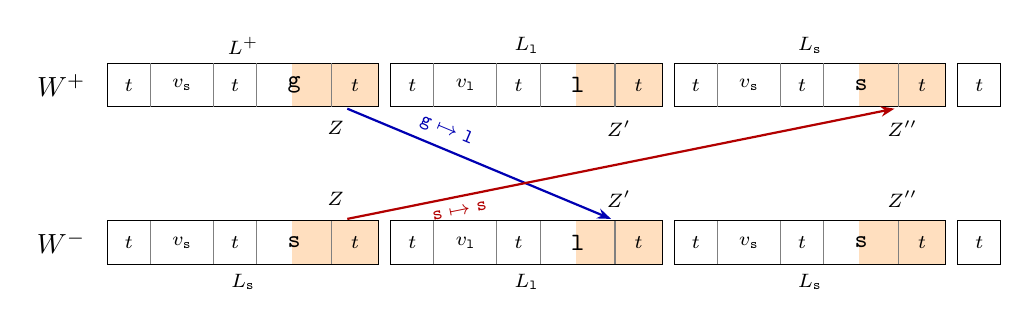
\begin{tikzpicture}[x=1cm,y=1cm,
    cellbox/.style={draw,minimum height=0.55cm,inner sep=0pt,font=\scriptsize},
    zone/.style={fill=orange!25},
    match/.style={-{Stealth[length=5pt]},thick}]
  % a block t v t c t starting at x=#1, row y=#2, displayed letter #3, name prefix #4
  \newcommand{\block}[4]{%
    \begin{scope}[shift={(#1,#2)}]
      \fill[zone] (2.35,-0.275) rectangle (3.45,0.275);
      \draw (0,-0.275) rectangle (3.45,0.275);
      \foreach \a in {0.55,1.35,1.9,2.85}{\draw[gray] (\a,-0.275) -- (\a,0.275);}
      \node[font=\scriptsize] at (0.275,0) {$t$};
      \node[font=\scriptsize] at (0.95,0) {$v_{\bs}$};
      \node[font=\scriptsize] at (1.625,0) {$t$};
      \node[font=\small] at (2.375,0) {#3};
      \node[font=\scriptsize] at (3.15,0) {$t$};
      \coordinate (#4) at (2.9,0);
    \end{scope}}
  \newcommand{\blockl}[4]{%
    \begin{scope}[shift={(#1,#2)}]
      \fill[zone] (2.35,-0.275) rectangle (3.45,0.275);
      \draw (0,-0.275) rectangle (3.45,0.275);
      \foreach \a in {0.55,1.35,1.9,2.85}{\draw[gray] (\a,-0.275) -- (\a,0.275);}
      \node[font=\scriptsize] at (0.275,0) {$t$};
      \node[font=\scriptsize] at (0.95,0) {$v_{\bl}$};
      \node[font=\scriptsize] at (1.625,0) {$t$};
      \node[font=\small] at (2.375,0) {#3};
      \node[font=\scriptsize] at (3.15,0) {$t$};
      \coordinate (#4) at (2.9,0);
    \end{scope}}
  % rows
  \node[anchor=east] at (-0.15,2) {$W^{+}$};
  \node[anchor=east] at (-0.15,0) {$W^{-}$};
  % W+ : L+ L_l L_s t
  \block{0}{2}{$\bg$}{P1}
  \blockl{3.6}{2}{$\bl$}{P2}
  \block{7.2}{2}{$\bs$}{P3}
  \draw (10.8,1.725) rectangle (11.35,2.275); \node[font=\scriptsize] at (11.075,2) {$t$};
  % W- : L_s L_l L_s t
  \block{0}{0}{$\bs$}{M1}
  \blockl{3.6}{0}{$\bl$}{M2}
  \block{7.2}{0}{$\bs$}{M3}
  \draw (10.8,-0.275) rectangle (11.35,0.275); \node[font=\scriptsize] at (11.075,0) {$t$};
  % block labels
  \foreach \x/\l in {1.725/{$L^{+}$},5.325/{$L_{\bl}$},8.925/{$L_{\bs}$}}{\node[font=\scriptsize] at (\x,2.5) {\l};}
  \foreach \x/\l in {1.725/{$L_{\bs}$},5.325/{$L_{\bl}$},8.925/{$L_{\bs}$}}{\node[font=\scriptsize] at (\x,-0.5) {\l};}
  % zone names
  \node[font=\scriptsize] at (2.9,1.45) {$Z$};
  \node[font=\scriptsize] at (6.5,1.45) {$Z'$};
  \node[font=\scriptsize] at (10.1,1.45) {$Z''$};
  \node[font=\scriptsize] at (2.9,0.55) {$Z$};
  \node[font=\scriptsize] at (6.5,0.55) {$Z'$};
  \node[font=\scriptsize] at (10.1,0.55) {$Z''$};
  % matchings
  \draw[match,blue!70!black] ($(P1)+(0.15,-0.3)$) -- node[pos=0.35,above,sloped,font=\scriptsize]{$\bg \mapsto \bl$} ($(M2)+(-0.1,0.3)$);
  \draw[match,red!70!black] ($(M1)+(0.15,0.3)$) -- node[pos=0.2,below,sloped,font=\scriptsize]{$\bs \mapsto \bs$} ($(P3)+(-0.1,-0.3)$);
\end{tikzpicture}

    \caption{The words $W^{-}$ and $W^{+}$ with the critical zones $Z, Z', Z''$ (shaded).
      Before each displayed branch the prefix state is $e_P$, and after each block the suffix state is $e_Q$.
      Outside $Z$ every vertex is matched to itself.
      The vertices of $Z$ in $\M^{+}_q$ (good branch $\bg$) are matched to $Z'$ in $\M^{-}_q$ (long branch $\bl$).
      The vertices of $Z$ in $\M^{-}_q$ are matched to $Z''$ in $\M^{+}_q$ (both shifted branches $\bs$).}
    \label{figure: reset}
  \end{figure}

  \begin{claim}\label{claim: outside}
    For every interior $x \notin Z$: $(\lambda^{+}(x), \rho^{+}(x)) = (\lambda^{-}(x), \rho^{-}(x))$.
  \end{claim}
  \begin{claimproof}
    The suffixes $\M^{\pm}_q\range{x, v}$ coincide, because they contain no $\vc$-pair.
    So $\rho^{+}(x) = \rho^{-}(x)$.
    If $x$ is before $Z$, both changed $\vc$-targets lie after $x$, so $\M^{+}_q\range{u, x} = \M^{-}_q\range{u, x}$.
    If $x$ is after $Z$, then $\alpha^{\pm}_x = \pc(L^{\pm})\, \gamma$ with $L^{-} \defeq L_{\bs}$ and a common word $\gamma$.
    Since $\varphi(L^{+}) = \varphi(L_{\bs}) = e_P$, \Cref{lemma: prefixes} gives $\lambda^{+}(x) = \lambda^{-}(x)$.
  \end{claimproof}

  \begin{claim}\label{claim: good to long}
    Let $x \in Z$ and let $x' \in Z'$ be its match.
    Then $(\lambda^{+}(x), \rho^{+}(x)) = (\lambda^{-}(x'), \rho^{-}(x'))$.
  \end{claim}
  \begin{claimproof}
    The displayed letters are $\bg$ (block one of $W^{+}$) and $\bl$ (block two of $W^{-}$).
    The words $\zeta_x$ and $\zeta_{x'}$ are one of the following pairs.
    (a) The prefixes of lengths $m-1$ of $\pc(\bg)$ and $m$ of $\pc(\bl)$.
    (b) The words $\pc(\bg)$ and $\pc(\bl)$.
    (c) The words $\pc(\bg)\,\delta$ and $\pc(\bl)\,\delta$ for a common prefix $\delta$ of $\pc(t)$.
    In each case $\tau_q(\zeta_x) = \tau_q(\zeta_{x'})$ by \Cref{lemma: branch identities}(\ref{item: long}) and \Cref{lemma: word types}(\ref{item: composition}).
    The words $\xi_x$ and $\xi_{x'}$ are equal.
    They are $00\,\scode(t)$ or $0\,\scode(t)$ in the branch, since $m \ge 3$ and the last two vertices are not first vertices of the branch.
    In the copy of $t$ they are the same suffix of $\scode(t)$.
    By \eqref{equation: zone states} and \Cref{lemma: prefixes,lemma: suffixes}, the claim follows.
  \end{claimproof}

  \begin{claim}\label{claim: shifted to shifted}
    Let $x \in Z$ and let $x'' \in Z''$ be its match.
    Then $(\lambda^{-}(x), \rho^{-}(x)) = (\lambda^{+}(x''), \rho^{+}(x''))$.
  \end{claim}
  \begin{claimproof}
    Both displayed letters are $\bs$.
    Hence $\zeta_x = \zeta_{x''}$ and $\xi_x = \xi_{x''}$, and we conclude by \eqref{equation: zone states} as before.
  \end{claimproof}

  By \Cref{claim: outside,claim: good to long}, $\Spec{q}(\M^{+}_q) \subseteq \Spec{q}(\M^{-}_q)$.
  By \Cref{claim: outside,claim: shifted to shifted}, $\Spec{q}(\M^{-}_q) \subseteq \Spec{q}(\M^{+}_q)$.
  Together with the root types, $\M^{+}_q \eqq{q} \M^{-}_q$.
\end{proof}

\begin{remark}
  The term $\Kt$ itself has star height one and distinguishes $\M^{+}_q$ from $\M^{-}_q$.
  So $\eqq{q}$ does not imply equivalence for all terms of star height one.
  What $\eqq{q}$ does guarantee is that stars of depth at most $q$ \emph{passing through} a module do not see the difference (\Cref{lemma: replacement}).
  The amplification in \Cref{section: cells} makes this enough.
  The suffix monoid $\Qm$ may contain nontrivial groups, for instance because $(\vr \compo \vr)^{*}$ counts modulo two.
  This is why we need the minimal ideal and the inverses $v_x$, and not only the aperiodicity of the prefix monoid.
\end{remark}

\section{Cells and parity}\label{section: cells}

Fix $q$ and the modules $\M^{+} \defeq \M^{+}_q$, $\M^{-} \defeq \M^{-}_q$ of \Cref{proposition: local pair}.
For a bit $\theta \in \set{0, 1}$, let $\M^{(1)} \defeq \M^{+}$ and $\M^{(0)} \defeq \M^{-}$.
So the bit of a module is the truth value of $\Kt(u, v)$.

\begin{definition}[Cell models]\label{definition: cells}
  Let $w = w_1 \cdots w_n \in \set{0,1}^{+}$.
  The valuation $\C(w)$ consists of the following vertices, ordered from left to right:
  \[
    p^{0}_{0} < p^{0}_{1} < \underbrace{u_1 < \cdots < v_1}_{\text{copy of } \M^{(w_1)}} < p^{1}_{0} < p^{1}_{1} < \underbrace{u_2 < \cdots < v_2}_{\text{copy of } \M^{(w_2)}} < \cdots < v_n < p^{n}_{0} < p^{n}_{1}.
  \]
  The relations $\vr, \vc, \vb$ are the union of the relations of the copies of the modules.
  The vertices $p^{i}_{0}, p^{i}_{1}$ are called \emph{ports}.
  Cell $i$ consists of the module $\range{u_i, v_i}$ together with its input ports $p^{i-1}_{0}, p^{i-1}_{1}$ and output ports $p^{i}_{0}, p^{i}_{1}$.
\end{definition}

No input pair leaves a module, and every input pair is strict.
So $\C(w)$ is an $\RSUB$ valuation with irreflexive $\vr, \vc, \vb$.

\begin{lemma}\label{lemma: cells pathwidth}
  $\pw(\C(w)) = 2$.
\end{lemma}
\begin{proof}
  We concatenate path decompositions.
  For each $i$, take the bags $\set{p^{i-1}_0, p^{i-1}_1}$ and $\set{p^{i-1}_1, u_i}$.
  Then take the bags of \Cref{lemma: module shape} for the $i$-th module, and finally the bag $\set{v_i, p^{i}_0}$.
  At the end we add the bag $\set{p^{n}_0, p^{n}_1}$.
  Every vertex occurs in an interval of bags, and every edge is covered, since the ports are joined only by successor pairs.
  All bags have at most three elements.
  The path from $u_1$ to $v_1$ together with the edge $\set{u_1, v_1}$ forms a cycle, so the pathwidth is at least two.
\end{proof}

\begin{figure}[t]
  \centering
  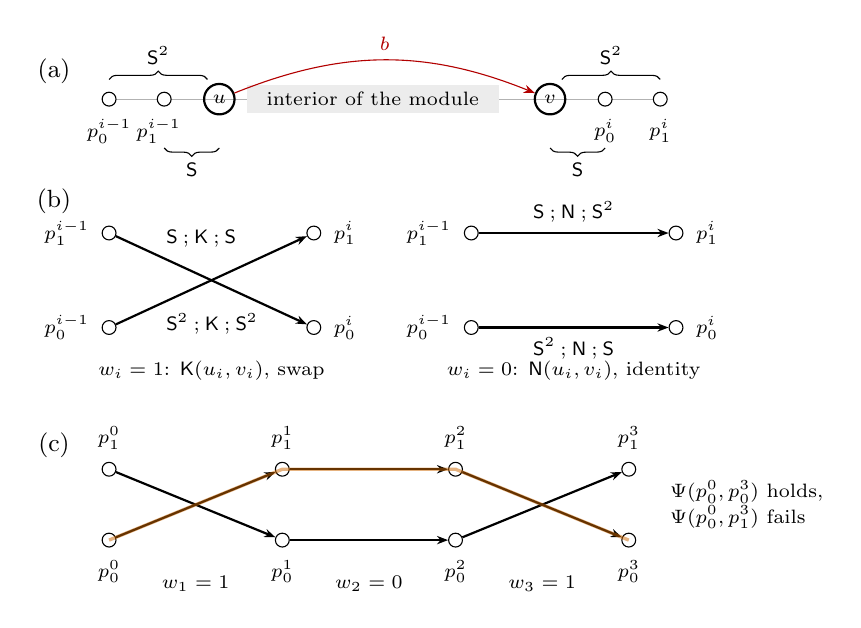
\begin{tikzpicture}[x=1cm,y=1cm,
    port/.style={circle,draw,fill=white,inner sep=0pt,minimum size=5pt},
    endpt/.style={circle,draw,thick,inner sep=0.5pt,minimum size=11pt,font=\scriptsize},
    harr/.style={-{Stealth[length=4pt]},thick},
    succ/.style={gray!60,thin}]
  % ---------- (a) order of the vertices in one cell ----------
  \node[font=\small] at (-0.7,0.35) {(a)};
  \draw[succ] (0,0) -- (7.0,0);
  \node[port] (a0) at (0,0) {}; \node[port] (a1) at (0.7,0) {};
  \node[endpt] (u) at (1.4,0) {$u$};
  \fill[gray!15] (1.75,-0.18) rectangle (4.95,0.18);
  \node[font=\scriptsize] at (3.35,0) {interior of the module};
  \node[endpt] (v) at (5.6,0) {$v$};
  \node[port] (b0) at (6.3,0) {}; \node[port] (b1) at (7.0,0) {};
  \node[font=\scriptsize,below=1pt] at (a0.south) {$p^{i-1}_0$};
  \node[font=\scriptsize,below=1pt,xshift=-2pt] at (a1.south) {$p^{i-1}_1$};
  \node[font=\scriptsize,below=1pt] at (b0.south) {$p^{i}_0$};
  \node[font=\scriptsize,below=1pt] at (b1.south) {$p^{i}_1$};
  \draw[red!70!black,-{Stealth[length=4pt]}] (u) to[bend left=22] node[above,font=\scriptsize]{$\vb$} (v);
  \draw[decorate,decoration={brace,amplitude=3pt}] (0,0.25) -- (1.25,0.25) node[midway,above=2pt,font=\scriptsize]{$\St^{2}$};
  \draw[decorate,decoration={brace,mirror,amplitude=3pt}] (0.7,-0.62) -- (1.4,-0.62) node[midway,below=2pt,font=\scriptsize]{$\St$};
  \draw[decorate,decoration={brace,amplitude=3pt}] (5.75,0.25) -- (7.0,0.25) node[midway,above=2pt,font=\scriptsize]{$\St^{2}$};
  \draw[decorate,decoration={brace,mirror,amplitude=3pt}] (5.6,-0.62) -- (6.3,-0.62) node[midway,below=2pt,font=\scriptsize]{$\St$};
  % ---------- (b) H-edges of one cell, two tracks ----------
  \begin{scope}[shift={(0,-2.9)}]
    \node[font=\small] at (-0.7,1.6) {(b)};
    \foreach \x/\bit/\K in {0/1/\Kt, 4.6/0/\Nt}{
      \begin{scope}[shift={(\x,0)}]
        \node[port] (l0) at (0,0) {}; \node[port] (l1) at (0,1.2) {};
        \node[port] (r0) at (2.6,0) {}; \node[port] (r1) at (2.6,1.2) {};
        \node[font=\scriptsize,left=1pt] at (l0.west) {$p^{i-1}_0$};
        \node[font=\scriptsize,left=1pt] at (l1.west) {$p^{i-1}_1$};
        \node[font=\scriptsize,right=1pt] at (r0.east) {$p^{i}_0$};
        \node[font=\scriptsize,right=1pt] at (r1.east) {$p^{i}_1$};
        \ifnum\bit=1
          \draw[harr] (l0) -- node[pos=0.22,below right=-1pt,font=\scriptsize]{$\St^{2}\compo\Kt\compo\St^{2}$} (r1);
          \draw[harr] (l1) -- node[pos=0.22,above right=-1pt,font=\scriptsize]{$\St\compo\Kt\compo\St$} (r0);
          \node[font=\scriptsize] at (1.3,-0.55) {$w_i = 1$: $\Kt(u_i, v_i)$, swap};
        \else
          \draw[harr] (l0) -- node[below,font=\scriptsize]{$\St^{2}\compo\Nt\compo\St$} (r0);
          \draw[harr] (l1) -- node[above,font=\scriptsize]{$\St\compo\Nt\compo\St^{2}$} (r1);
          \node[font=\scriptsize] at (1.3,-0.55) {$w_i = 0$: $\Nt(u_i, v_i)$, identity};
        \fi
      \end{scope}
    }
  \end{scope}
  % ---------- (c) two-track view of C(101) ----------
  \begin{scope}[shift={(0,-5.6)}]
    \node[font=\small] at (-0.7,1.2) {(c)};
    \foreach \i in {0,1,2,3}{
      \node[port] (q\i0) at (2.2*\i,0) {};
      \node[port] (q\i1) at (2.2*\i,0.9) {};
      \node[font=\scriptsize,below=1pt] at (q\i0.south) {$p^{\i}_0$};
      \node[font=\scriptsize,above=1pt] at (q\i1.north) {$p^{\i}_1$};
    }
    \foreach \i/\j/\b in {0/1/1,1/2/0,2/3/1}{
      \ifnum\b=1
        \draw[harr] (q\i0) -- (q\j1); \draw[harr] (q\i1) -- (q\j0);
      \else
        \draw[harr] (q\i0) -- (q\j0); \draw[harr] (q\i1) -- (q\j1);
      \fi
      \node[font=\scriptsize] at (2.2*\i+1.1,-0.55) {$w_{\j}=\b$};
    }
    \draw[very thick,orange!80!black,opacity=0.5] (q00.center) -- (q11.center) -- (q21.center) -- (q30.center);
    \node[font=\scriptsize,anchor=west,align=left] at (7.0,0.45) {$\Psit(p^0_0,p^3_0)$ holds,\\ $\Psit(p^0_0,p^3_1)$ fails};
  \end{scope}
\end{tikzpicture}

  \caption{(a) The order of the vertices in cell $i$; the braces show the shifts by $\St$ and $\St^{2}$ used in $\Ht$.
    (b) The edges of $\Ht$ in cell $i$, drawn on two tracks.
    A module in $\Kt$ (bit $1$) swaps the ports, and a module in $\Nt$ (bit $0$) keeps them.
    (c) The edges of $\Ht$ in $\C(101)$.
    The highlighted $\Ht$-path from $p^{0}_{0}$ uses two swaps and ends in $p^{3}_{0}$.
    In general, $\Psit(p^{0}_{0}, p^{n}_{1})$ holds iff the number of swaps is odd.}
  \label{figure: cells}
\end{figure}

\begin{lemma}[Parity]\label{lemma: parity}
  In $\C(w)$, the relation $\Ht$ is exactly
  \[
    \set{(p^{i-1}_{j}, p^{i}_{j \oplus w_i}) \mid i \in \range{n},\ j \in \set{0, 1}},
  \]
  where $\oplus$ is addition modulo two.
  Consequently, $\Psit(p^{0}_{0}, p^{n}_{1})$ holds in $\C(w)$ iff the number of $1$s in $w$ is odd.
\end{lemma}
\begin{proof}
  The relation $\vb$ consists of the pairs $(u_i, v_i)$.
  By \Cref{lemma: locality}, $\Kt(u_i, v_i)$ is evaluated in the $i$-th module, so it holds iff $w_i = 1$.
  Hence $\Kt = \set{(u_i, v_i) \mid w_i = 1}$ and $\Nt = \set{(u_i, v_i) \mid w_i = 0}$.
  The only vertex $x$ with $\St^{2}(x, u_i)$ is $p^{i-1}_0$, and the only vertex with $\St(x, u_i)$ is $p^{i-1}_1$.
  Similarly, the only $y$ with $\St(v_i, y)$ is $p^{i}_0$, and the only $y$ with $\St^{2}(v_i, y)$ is $p^{i}_1$.
  Reading off \eqref{equation: Psi} gives the description of $\Ht$; see \Cref{figure: cells}(a,b).
  Every $\Ht$-path from $p^{0}_{0}$ passes through one port of each layer $i$.
  It changes the index exactly at the cells with $w_i = 1$.
\end{proof}

\section{Replacing a module}\label{section: replacement}

\begin{lemma}[Seams]\label{lemma: seam}
  For every star-free term $G$ there is a finite set $\mathcal{R}(G)$ of pairs $(A, C)$ of star-free terms with the following properties.
  We have $\cd(A), \cd(C) \le \cd(G)$ for all pairs.
  Moreover, let $\A$ be a valuation and $x \le c \le y$ such that no input pair $(a, a')$ satisfies $x \le a < c < a' \le y$.
  Then
  \[
    G(x, y) \iff \bigvee_{(A, C) \in \mathcal{R}(G)} A(x, c) \wedge C(c, y).
  \]
\end{lemma}
\begin{proof}
  By induction on $G$.
  For a variable $o \in \set{\vr, \vc, \vb}$ we take $\set{(\id, o), (o, \id)}$.
  If $x < c < y$, then $o(x, y)$ fails by assumption, and if $c \in \set{x, y}$, one of the two pairs applies.
  For $\id$ we take $\set{(\id, \id)}$, and for $\emp$ the empty set.
  For Boolean operations, let $\mathcal{A}$ and $\mathcal{C}$ be the sets of first and second components occurring in the pairs of the subterms.
  The atoms of the finite Boolean algebras generated by $\mathcal{A}$ and by $\mathcal{C}$ are Boolean combinations of terms of depth at most $\cd(G)$.
  Every Boolean combination of the subterms is a union of products of such atoms.
  For complement this uses that $\topr(x, y)$ holds for $x \le y$.
  For $G = G_1 \compo G_2$, split on whether the intermediate point $z$ satisfies $z \le c$ or $z \ge c$.
  If $z \le c$, the interval $\range{z, y}$ again satisfies the hypothesis, so $G_2(z, y)$ decomposes at $c$.
  This gives the pairs $(G_1 \compo A_2, C_2)$ for $(A_2, C_2) \in \mathcal{R}(G_2)$.
  Symmetrically, $z \ge c$ gives $(A_1, C_1 \compo G_2)$ for $(A_1, C_1) \in \mathcal{R}(G_1)$.
  In both cases the depth is at most $\max(\cd(G_1), \cd(G_2)) + 1$.
\end{proof}

\begin{lemma}[Replacement]\label{lemma: replacement}
  Let $\A, \A'$ be valuations on the same linear order $V$, and let $u < v$ in $V$.
  Let $O \defeq V \setminus \set{z \mid u < z < v}$ be the set of \emph{outer} vertices.
  Assume the following.
  \begin{enumerate}
    \item\label{item: same outside} $\A$ and $\A'$ have the same input pairs inside $O \times O$.
    \item\label{item: isolated} In neither valuation does an input pair have one component in $\set{z \mid u < z < v}$ and the other in $O \setminus \set{u, v}$.
    \item\label{item: local equivalence} $\A\range{u, v} \eqq{q} \A'\range{u, v}$.
  \end{enumerate}
  Then for all $F \in \SF{q}$ and $x, y \in O$: $F(x, y)$ holds in $\A$ iff it holds in $\A'$, and the same holds for $F^{*}(x, y)$.
\end{lemma}
\begin{proof}
  \emph{Star-free terms.}
  We use induction on $F \in \SF{q}$.
  Atoms are handled by (\ref{item: same outside}), and Boolean operations are immediate.
  Let $F = G_1 \compo G_2$ with $\cd(G_1), \cd(G_2) \le q - 1$, and let $x \le z \le y$.
  If $z \in O$, we use the induction hypothesis for $G_1(x, z)$ and $G_2(z, y)$.
  Otherwise $x \le u < z < v \le y$.
  By (\ref{item: isolated}), \Cref{lemma: seam} applies to $G_1(x, z)$ at the seam $u$ and to $G_2(z, y)$ at the seam $v$.
  So the existence of such a $z$ is equivalent to
  \[
    \bigvee_{(A_1, C_1) \in \mathcal{R}(G_1)}\ \bigvee_{(A_2, C_2) \in \mathcal{R}(G_2)}
      A_1(x, u) \wedge \bigl((C_1 \inter \Dt) \compo (A_2 \inter \Dt)\bigr)(u, v) \wedge C_2(v, y).
  \]
  The intervals $\range{x, u}$ and $\range{v, y}$ consist of outer vertices.
  By (\ref{item: same outside}) and \Cref{lemma: locality}, the values of $A_1(x, u)$ and $C_2(v, y)$ agree in $\A$ and $\A'$.
  The middle conjunct is evaluated in $\range{u, v}$ by a term of depth at most $q$.
  So it agrees by \Cref{lemma: spectrum}.

  \emph{Stars.}
  Let $F^{*}(x, y)$ hold in $\A$, witnessed by $x = x_0 < x_1 < \dots < x_k = y$ with $F(x_{i-1}, x_i)$.
  We may drop repeated points, since all values are forward.
  If no $x_i$ is in the interior, the path transfers to $\A'$ by the first part.
  Otherwise the interior points form a block $x_s, \dots, x_t$ with $1 \le s \le t \le k - 1$.
  Let $a \defeq x_{s-1} \le u$ and $b \defeq x_{t+1} \ge v$.
  By \Cref{lemma: seam} at $u$ and $v$, there are $(A_1, C_1), (A_2, C_2) \in \mathcal{R}(F)$ with the following properties.
  $A_1(a, u)$ and $C_2(v, b)$ hold, and so does the observation
  \[
    \bigl((C_1 \inter \Dt) \compo F^{*} \compo (A_2 \inter \Dt)\bigr)(u, v).
  \]
  These terms lie in $\SF{q}$.
  By \Cref{lemma: spectrum} the observation also holds in $\A'\range{u, v}$, which gives interior $z \le z'$ there.
  By \Cref{lemma: seam} in $\A'$, we get $F(a, z)$ and $F(z', b)$.
  Here $A_1(a, u)$ and $C_2(v, b)$ are unchanged by (\ref{item: same outside}).
  The parts $x_0, \dots, x_{s-1}$ and $x_{t+1}, \dots, x_k$ consist of outer vertices and transfer by the first part.
  So $F^{*}(x, y)$ holds in $\A'$.
  The converse direction is symmetric.
\end{proof}

\section{Ruling out star height one}\label{section: lower bound}

We prove \Cref{theorem: lower bound}.
Let $E$ be a term with $\sh(E) \le 1$.
Every star in $E$ has the form $F^{*}$ with $F$ star-free.
Let $q$ be at least $\cd(F)$ for all subterms $F^{*}$ of $E$.
Take the modules $\M^{\pm} = \M^{\pm}_q$ of \Cref{proposition: local pair} and the cell models $\C(w)$ of \Cref{definition: cells}.

\subparagraph*{Coordinates.}
Let $\mathbb{V}$ be the common vertex set of $\M^{+}$ and $\M^{-}$, and let $\Theta \defeq \mathbb{V} \uplus \set{\pi_0, \pi_1}$ be the set of \emph{tags}.
For $w = w_1 \cdots w_n$, let $\hat w \defeq {\triangleright}\, w$ be the word over $\Lambda \defeq \set{{\triangleright}, 0, 1}$ with positions $0, \dots, n$.
We call $\set{p^{0}_0, p^{0}_1}$ \emph{block $0$}.
For $i \ge 1$, \emph{block $i$} is $\range{u_i, v_i} \cup \set{p^{i}_0, p^{i}_1}$.
A vertex of $\C(w)$ in block $i$ gets the coordinates $(i, \vartheta)$.
Here $\vartheta \in \mathbb{V}$ is its vertex in the module, or $\pi_j$ if it is the port $p^{i}_j$.
Order $\Theta$ by the order of $\mathbb{V}$ followed by $\pi_0 < \pi_1$.
Then the order of $\C(w)$ is the lexicographic order of coordinates.

\begin{lemma}[Normalization]\label{lemma: normalization}
  Let $F^{*}$ be a subterm of $E$, and let $x = (i, \vartheta)$ and $y = (j, \vartheta')$ be vertices of $\C(w)$ with $x \le y$.
  Then the truth value of $F^{*}(x, y)$ in $\C(w)$ depends only on $\vartheta, \vartheta', \hat w_i, \hat w_j$ and $j - i$.
\end{lemma}
\begin{proof}
  Let $w'$ arise from $w$ by setting $w_k \defeq 0$ for every $k$ with $\range{u_k, v_k} \subseteq \range{x, y}$.
  We pass from $\C(w)$ to $\C(w')$ one module at a time.
  Each step replaces a copy of $\M^{+}$ by a copy of $\M^{-}$ in an interval $\range{u_k, v_k} \subseteq \range{x, y}$.
  The conditions of \Cref{lemma: replacement} hold.
  (\ref{item: same outside}) holds since the modules differ only in a $\vc$-pair with an interior target.
  (\ref{item: isolated}) holds since no input pair leaves a module.
  (\ref{item: local equivalence}) holds by \Cref{proposition: local pair}.
  Moreover, $x$ and $y$ are outer.
  So $F^{*}(x, y)$ has the same value in $\C(w)$ and in $\C(w')$.
  In $\C(w')$ all modules strictly between blocks $i$ and $j$ are copies of $\M^{-}$.
  So by \Cref{lemma: locality}, the value is determined by $\vartheta, \vartheta'$, $w'_i, w'_j$ (when $i, j \ge 1$) and $j - i$.
  These are in turn determined by $\vartheta, \vartheta', \hat w_i, \hat w_j$ and $j - i$.
\end{proof}

For a subterm $F^{*}$ of $E$, let $f_F(\vartheta, a, \vartheta', a', k) \in \set{0,1}$ be the value given by \Cref{lemma: normalization}, for $a, a' \in \Lambda$ and $k \ge 0$.

\begin{lemma}[Periodicity]\label{lemma: periodicity}
  There are $N_0 \in \nat$ and $d \ge 1$ such that $f_F(\vartheta, a, \vartheta', a', k) = f_F(\vartheta, a, \vartheta', a', k + d)$ for all subterms $F^{*}$ of $E$, all $\vartheta, a, \vartheta', a'$ and all $k \ge N_0$.
\end{lemma}
\begin{proof}
  Since there are finitely many choices of $F, \vartheta, a, \vartheta', a'$, it suffices to show that each sequence $k \mapsto f_F(\vartheta, a, \vartheta', a', k)$ is ultimately periodic.
  For $k \ge 1$, the normalized interval $\range{x, y}$ in the proof of \Cref{lemma: normalization} is an ordered sum $X \oplus B^{k-1} \oplus Y$.
  Here $X$ is the rest of block $i$ from $x$, $B$ is a copy of $\M^{-}$ followed by two ports, and $Y$ is the part of block $j$ up to $y$.
  No input pair connects different summands.
  Write the vertices of $X$, $B$ and $Y$ as letters of a finite alphabet, using disjoint copies.
  Then $X \oplus B^{k-1} \oplus Y$ is first-order interpretable in the word that lists its vertices.
  Two positions lie in the same summand iff their distance equals the distance of their letters inside that summand, and this is first-order expressible with a bounded number of successor steps.
  Since $F^{*}$ is definable in monadic second-order logic, the set of $k$ for which $F^{*}(\min, \max)$ holds is the preimage of a regular language under $k \mapsto \delta_X \delta_B^{k-1} \delta_Y$~\cite{buchiWeakSecondorderArithmetic1960}.
  Hence it is ultimately periodic.
\end{proof}

\subparagraph*{Translation into first-order logic with modular predicates.}
Let $\FO[<, \MOD{d}]$ be first-order logic over words in $\Lambda^{*}$.
It has the order, a unary predicate $P_a$ for each $a \in \Lambda$, and unary predicates $\mathrm{mod}^{r}_{d}(i)$, meaning $i \equiv r \pmod d$, for $r \in \range{0, d-1}$.
Expressions such as $j = i + k$ for a constant $k$, $j \ge i + N_0$, and $j - i \equiv r \pmod d$ are definable.
The last one is $\bigvee_{r'} \mathrm{mod}^{r'}_d(i) \wedge \mathrm{mod}^{r' + r}_d(j)$.

\begin{lemma}[Translation]\label{lemma: translation}
  For every subterm $G$ of $E$ and all tags $\vartheta, \vartheta' \in \Theta$, there is an $\FO[<, \MOD{d}]$ formula $\varphi^{\vartheta, \vartheta'}_{G}(i, j)$ with the following property.
  For all $w \in \set{0,1}^{+}$ and all vertices $(i, \vartheta) \le (j, \vartheta')$ of $\C(w)$, we have $G((i, \vartheta), (j, \vartheta'))$ in $\C(w)$ iff $\hat w \models \varphi^{\vartheta, \vartheta'}_{G}(i, j)$.
\end{lemma}
\begin{proof}
  By induction on $G$.
  Let $\mathrm{vert}_{\vartheta}(i)$ express that $(i, \vartheta)$ is a vertex, that is, $i > 0$ or $\vartheta \in \set{\pi_0, \pi_1}$.
  Let $\mathrm{le}_{\vartheta,\vartheta'}(i, j)$ express $(i, \vartheta) \le (j, \vartheta')$.
  \begin{itemize}
    \item Variables $o \in \set{\vr, \vc, \vb}$: every input pair lies in one module, so we take $i = j \wedge \bigvee \set{P_a(i) \mid a \in \set{0,1},\ (\vartheta, \vartheta') \in o^{\M^{(a)}}}$.
          The constants $\id$ and $\emp$ are similar.
    \item $\com{G}$: take $\mathrm{le}_{\vartheta,\vartheta'}(i, j) \wedge \neg\varphi^{\vartheta, \vartheta'}_{G}$, and $G_1 \union G_2$: take the disjunction.
    \item $G_1 \compo G_2$: take $\exists k \bigvee_{\vartheta''} (\mathrm{vert}_{\vartheta''}(k) \wedge \varphi^{\vartheta, \vartheta''}_{G_1}(i, k) \wedge \varphi^{\vartheta'', \vartheta'}_{G_2}(k, j))$.
    \item $F^{*}$: by \Cref{lemma: normalization,lemma: periodicity}, take the disjunction over $a, a' \in \Lambda$ of $P_a(i) \wedge P_{a'}(j) \wedge \psi_{a, a'}(i, j)$.
          Here $\psi_{a, a'}$ is the disjunction of the following formulas.
          First, $j = i + k$ for each $k < N_0$ with $f_F(\vartheta, a, \vartheta', a', k) = 1$.
          Second, $j \ge i + N_0 \wedge j - i \equiv r \pmod d$ for each $r$ such that $f_F(\vartheta, a, \vartheta', a', k) = 1$ for the $k \ge N_0$ with $k \equiv r$.
          \qedhere
  \end{itemize}
\end{proof}

\begin{lemma}[Parity is not definable]\label{lemma: parity undefinable}
  No $\FO[<, \MOD{d}]$ sentence $\varphi$ satisfies, for all $w \in \set{0,1}^{+}$: ${\triangleright} w \models \varphi$ iff $w$ has an odd number of $1$s.
\end{lemma}
\begin{proof}
  Restrict to $w = (1\, 0^{d-1})^{n}$, which has $n$ ones.
  The word ${\triangleright} w$ has positions $0, \dots, nd$.
  It is first-order interpretable in the linear order $\range{0, n}$ with $d$ copies.
  Position $0$ is $(0, 0)$, and position $(k-1)d + r + 1$ is $(k, r)$ for $k \in \range{n}$ and $r \in \range{0, d-1}$.
  The order is lexicographic.
  $P_{\triangleright}$ holds iff $k = 0$, $P_1$ iff $k \ne 0$ and $r = 0$, and $P_0$ iff $k \ne 0$ and $r \ne 0$.
  $\mathrm{mod}^{r'}_d$ holds at $(k, r)$ with $k \ne 0$ iff $r + 1 \equiv r' \pmod d$.
  All of these are first-order definable in $(\range{0, n}, <)$.
  Hence $\varphi$ would yield a first-order sentence $\varphi^{\flat}$ such that $(\range{0, n}, <) \models \varphi^{\flat}$ iff $n$ is odd.
  But linear orders of size at least $2^{\ell}$ are indistinguishable by sentences of quantifier rank $\ell$~\cite{ebbinghausFiniteModelTheory1995}.
\end{proof}

\begin{proof}[Proof of \Cref{theorem: lower bound}]
  Assume that $E$ is equivalent to $\Psit$ on $\Cls{2}$.
  Every $\C(w)$ lies in $\Cls{2}$ by \Cref{lemma: cells pathwidth}, and its relations are irreflexive.
  By \Cref{lemma: parity}, $E((0, \pi_0), (n, \pi_1))$ holds in $\C(w)$ iff $w$ has an odd number of $1$s.
  By \Cref{lemma: translation}, this property is defined by the sentence $\exists i\, \exists j\, (i \text{ is first} \wedge j \text{ is last} \wedge \varphi^{\pi_0, \pi_1}_{E}(i, j))$, contradicting \Cref{lemma: parity undefinable}.
\end{proof}

\begin{remark}\label{remark: more variables}
  The proof does not use that $E$ is a term over $\vr, \vc, \vb$ only.
  If $E$ contains further variables, we interpret them as empty in $\C(w)$.
  This changes neither the graph nor any argument above.
  So $\Psit$ is not equivalent on $\Cls{2}$ to any term of star height at most one, over any finite set of variables.
\end{remark}

\section{Pathwidth one}\label{section: pathwidth one}

\begin{lemma}\label{lemma: pathwidth one pairs}
  Let $\A$ be a valuation with $\pw(\A) \le 1$.
  Then every input pair $(x, y)$ satisfies $x = y$ or $y = \succrel(x)$.
\end{lemma}
\begin{proof}
  Suppose $x < y$ and $y \ne \succrel(x)$.
  Then the successor path from $x$ to $y$ together with the edge $\set{x, y}$ is a cycle in $\Gaif(\A)$.
  So $\Gaif(\A)$ is not a forest and has pathwidth at least two.
\end{proof}

\begin{proposition}\label{proposition: pathwidth one}
  Let $\Kt' \defeq \vb \inter ((\id \inter \vc) \compo \Dt)$ and $\Nt' \defeq \vb \setminus \Kt'$.
  Let $\Psit'$ be $\Psit$ with $\Kt, \Nt$ replaced by $\Kt', \Nt'$.
  Then $\sh(\Psit') = 1$, and $\Psit'$ is equivalent to $\Psit$ on $\Cls{1}$.
  In particular, $\gsh{\Cls{1}}(\Psit) \le 1$.
\end{proposition}
\begin{proof}
  It suffices to show $\Kt = \Kt'$ on every valuation $\A$ of pathwidth at most one.
  Both relations are contained in $\vb$ and are empty on the diagonal, since $(\cdots) \compo \Dt$ never holds at $(x, x)$.
  Let $\vb(x, y)$ with $x < y$.
  By \Cref{lemma: pathwidth one pairs}, $y = \succrel(x)$.
  So the only $z$ with $x \le z < y$ is $z = x$.
  Since $(\vr \compo \vr)^{*}(x, x)$ always holds, both $\Kt(x, y)$ and $\Kt'(x, y)$ are equivalent to $\vc(x, x)$.
\end{proof}

For strict valuations, $\Kt'$ is empty and $\Psit$ is equivalent on $\Cls{1}$ to $\bigl((\St^{2} \compo \vb \compo \St) \union (\St \compo \vb \compo \St^{2})\bigr)^{*}$.
Together with \Cref{theorem: lower bound}, the least pathwidth at which $\Psit$ needs star height two is exactly two.

\begin{remark}[Pathwidth one and words]\label{remark: pathwidth one words}
  By \Cref{lemma: pathwidth one pairs}, a valuation $\A \in \Cls{1}$ on $x_0 < \dots < x_n$ is given by two pieces of data.
  The first is the word $a_1 \cdots a_n$ over the alphabet $2^{\set{\vr, \vc, \vb}}$, where $a_k$ is the set of variables containing $(x_{k-1}, x_k)$.
  The second is the set of variables containing the diagonal.
  For each choice of the second datum, the following translations preserve the star height.
  A term then defines a regular language over $2^{\set{\vr, \vc, \vb}}$.
  Conversely, a regular expression with complement over this alphabet translates back into a term.
  For this, each letter $a$ becomes $\St \inter \bigcap_{o \in a} o \inter \bigcap_{o \notin a} \com{o}$, and the diagonal datum is tested by star-free terms such as $(\id \inter o) \compo \topr$.
  So the question whether heights one and two separate on $\Cls{1}$ is closely related to the generalized star-height problem for regular languages~\cite{pinResultsGeneralizedStarheight1992}.
  We do not work out the details of this correspondence here.
  % TODO: check whether to state the exact equivalence.
\end{remark}

\section{Conclusion}\label{section: conclusion}

We have shown that generalized star height two is needed already on $\RSUB$ valuations of pathwidth two.
The witness $\Psit$ uses three variables.
Its counter-models are paths with fans attached, and $\Psit$ itself collapses to star height one on pathwidth one.
The heart of the proof is \Cref{proposition: local pair}.
There, the aperiodicity of first-order types and an idempotent of the minimal ideal of a product monoid fool every star of bounded depth at once, even though the suffix monoid may count modulo a number.

We list some questions.
\begin{itemize}
  \item \emph{Higher levels.}
        Does the generalized star-height hierarchy relative to $\Cls{k}$ collapse for every fixed $k$?
        If it does not, how does the least pathwidth needed for a separation of heights $h$ and $h+1$ grow with $h$?
  \item \emph{Pathwidth one.}
        By \Cref{remark: pathwidth one words}, separating heights one and two on $\Cls{1}$ is closely related to the open generalized star-height problem for regular languages.
        Our construction does not apply there: it needs the edges from $u$ to the branches in order to keep the branches apart.
  \item \emph{Fewer variables.}
        Can the separation on $\Cls{2}$ be achieved with one or two variables?
  \item \emph{Other width measures.}
        The counter-models are outerplanar.
        Which structural restrictions, beyond pathwidth one, force a collapse?
\end{itemize}


\bibliography{main}

\end{document}
